Resumen de diferentes partes: 

- Ajuste de agentes -> LoRa? -> comentar lo de los agentes instruct.
- El protocolo MCP
- El estado del arte en arquitecturas de agentes LLM y sistemas RAG
- 
- El estado del arte en agentes integrados a proyectos software + contexto de onboarding ~quizás en la introducción.
- Redes neuronales?

2. Agentes LLM (Fundamentos y funcionamiento básico)

¿Qué son los agentes LLM?
2.1. Modelos LLM
2.2. Interacción con herramientas
2.3. Abstracciones en frameworks

\section{Agentes LLM}

Los agentes de Inteligencia Artificial son programas informáticos que implementan modelos computacionales avanzados para ejecutar diversas funciones específicas del contexto en el que se aplican. Tras siete décadas y media de investigación, los esfuerzos en el campo se han focalizado en agentes basados en Grandes Modelos de Lenguaje (LLM). 

Estos agentes, en esencia, constituyen sistemas informáticos que utilizan dichos modelos como núcleo operativo para la resolución de problemas. Para ello, les suministran los datos de entrada pertinentes, interpretan sus respuestas y transforman estas salidas en acciones concretas que permiten alcanzar los resultados deseados.

\subsection{Modelos LLM}

Los modelos de lenguaje (LM) constituyen sistemas computacionales especializados en el procesamiento del lenguaje natural. Entre estos, destacan los grandes modelos de lenguaje, diseñados para acometer tareas  como la clasificación y generación de contenido lingüístico. Su fundamento técnico reside en redes neuronales que implementan la arquitectura Transformer [Attention is All You Need]. Para comprender el funcionamiento de dicha arquitectura, resulta imprescindible asimilar previamente conceptos como la tokenización y las representaciones vectoriales del lenguaje.

\paragraph{Tokens}
Los tokens constituyen la unidad mínima de texto que el modelo puede procesar. Dado que operan sobre estructuras matemáticas, requieren transformar el lenguaje natural en representaciones matriciales. Para lograr esta conversión, el texto se segmenta en dichas unidades mínimas, que pueden corresponder a caracteres individuales, fragmentos de texto o palabras completas. El conjunto íntegro de estas unidades reconocibles por el modelo configura su vocabulario. 

\paragraph{Representaciones vectoriales}
Constituyen vectores numéricos de dimensionalidad fija que codifican la semántica inherente a cada token. Estos vectores pueden comprender desde 768 dimensiones en arquitecturas como BERT-base hasta superar las 16.000 dimensiones en los modelos más avanzados del estado del arte, capturando conceptos semánticos en profundidad. Por ejemplo, una dimensión específica podría especializarse en representar conceptos abstractos. En este contexto, la representación vectorial del token ``animal`` presentaría un valor más elevado en dicha dimensión que la correspondiente al término ``gato``, reflejando su mayor grado de abstracción conceptual.

\subsubsection{Arquitectura Transformer}
Esta arquitectura emplea el mecanismo de ``atención`` para enriquecer la comprensión textual del modelo. El proceso transforma inicialmente la representación de las palabras de entrada incorporando información contextual mediante múltiples capas de atención, que consisten en operaciones matriciales que transfieren información semántica entre palabras. 

Los agentes LLM utilizan predominantemente modelos decodificadores autorregresivos (GPT, Claude-Sonnet, Llama), optimizados para la generación secuencial de texto. Su característica distintiva es la aplicación de atención únicamente sobre tokens precedentes, permitiendo que el modelo compute la influencia de tokens anteriores sobre el actual sin modificar representaciones previas.

La figura \ref{fig:atencion_gato} ilustra un ejemplo simplificado del cómputo de atención para la frase ``El gato duerme``. Al generar la siguiente palabra, el modelo presta atención diferenciada a elementos previos, considerando más relevante que el gato esté durmiendo que su color. Así, calcula la probabilidad del siguiente token considerando todo el vocabulario disponible. Es importante destacar que, debido a la naturaleza autorregresiva, la influencia de un token posterior como ``negro`` no se aplica a tokens anteriores como ``gato``.

\begin{figure}
    \centering
    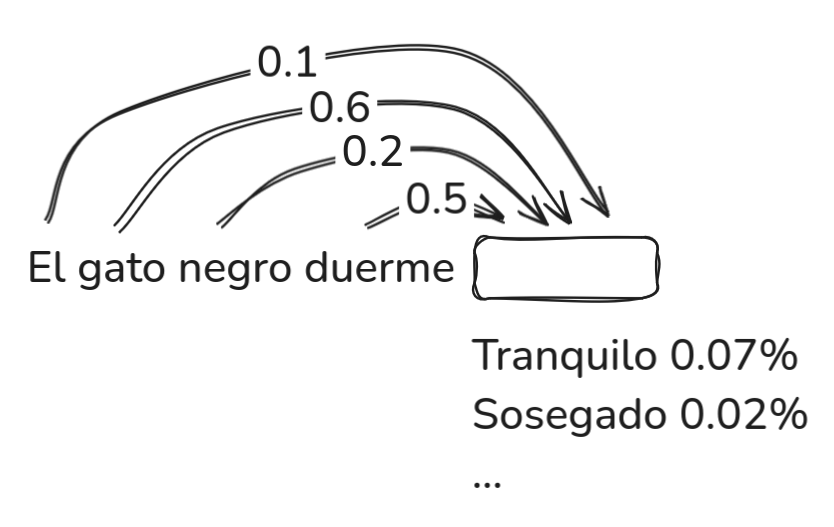
\includegraphics[width=0.65\linewidth]{figures/atencion_poc.png}
    \caption{Ejemplo simplificado de cómputo de atención para la frase \textquotedbl El gato duerme\textquotedbl}
    \label{fig:atencion_gato}
\end{figure}

En implementaciones prácticas, el mecanismo de atención que opera entre un token origen y un token destino se computa mediante operaciones matriciales que involucran tanto las representaciones vectoriales de ambos tokens como las matrices de atención, componentes de los parámetros aprendidos del modelo. Durante el proceso de entrenamiento, estas matrices de atención adquieren la capacidad de capturar fenómenos lingüísticos; por ejemplo, una matriz específica podría especializarse en cuantificar la connotación negativa que un token origen proyecta sobre un token destino.

\subsection{Interacción con herramientas externas}
Los agentes LLM poseen la capacidad de interactuar con diversas herramientas como búsquedas web, bases de datos o interfaces de usuario. Fundamentalmente, un LLM solo genera tokens de texto, por lo que la integración de herramientas se implementa mediante palabras clave que el modelo puede producir. Para ello, en el texto de entrada se especifica el esquema de la función a utilizar y, si decide emplearla, el modelo generará el texto correspondiente. Posteriormente, se procesa la respuesta para extraer llamadas a funciones si las hubiese.

La interacción con herramientas es típicamente alternante. Tras realizar la llamada a la herramienta, la salida de esta se utilizará como entrada para el siguiente mensaje del modelo. La figura \ref{fig:herramientas} ilustra el esquema de un agente con acceso a una API del clima. Como el modelo carece de información climática en tiempo real, se le indica en el prompt la posibilidad de invocar esta función. Al incluir la llamada en su texto de salida, se ejecuta la función y su respuesta se transmite al modelo para generar el resultado final.

\begin{figure}
  \centering
  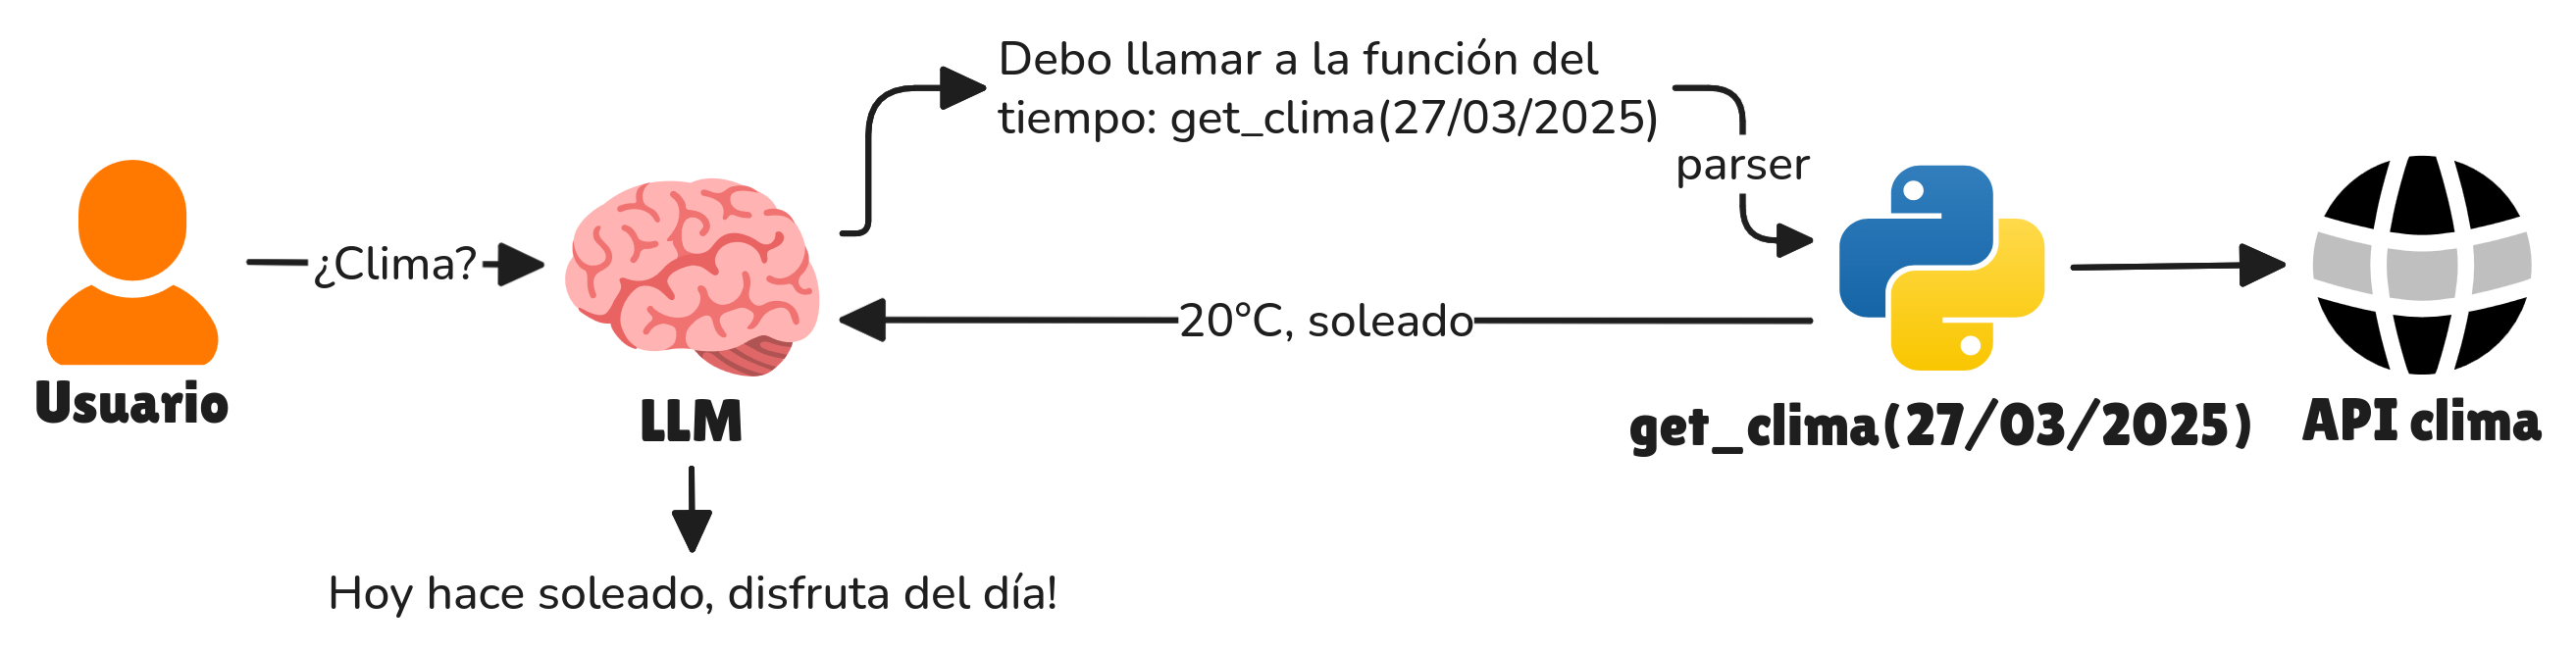
\includegraphics[width=1\linewidth]{figures/herramienta.png}
  \caption{Ejemplo de interacción de un modelo LLM con una herramienta externa.}
  \label{fig:herramientas}
\end{figure}

\subsection{Abstraciones en frameworks}
Aunque los agentes LLM son una tecnología de reciente surgimiento, ya se han desarrollado frameworks que estandarizan su implementación. Estas estructuras de trabajo, como LangChain o LangGraph, ofrecen abstracciones de alto nivel reutilizar funcionalidades comunes presentes en la mayoría de sistemas de agentes.
Las funcionalidades principales que estos frameworks proporcionan son:
\begin{itemize}
\item {\textbf{Gestión de modelos:}} La ejecución de modelos LLM requiere una comprensión profunda del modelo empleado. Cada LLM utiliza su propio tokenizador y está configurado para funcionar con un esquema específico de entrada y salida. Los frameworks simplifican esta complejidad, implementando una interfaz unificada que permite a los desarrolladores utilizar diversos modelos sin necesidad de profundizar en los detalles técnicos de su implementación.
\item {\textbf{Interacción conversacional:}} La comunicación con los modelos se efectúa mediante un esquema conversacional, donde el modelo recibe un texto de entrada y genera una respuesta correspondiente. Las respuestas y entradas se concatenan secuencialmente para preservar el contexto de la conversación, de manera que cada consulta subsiguiente incorpora todos los intercambios precedentes.
  \item {\textbf{Uso de herramientas externas:}} El desarrollador únicamente debe especificar la función que desea incorporar, toda la compljeidad de la interacción se abstrae en el framework.
\item {\textbf{Interacción entre agentes:}} Los agentes pueden establecer comunicación entre sí, permitiendo la construcción de sistemas con mayor complejidad. Numerosos frameworks establecen protocolos que definen las modalidades de comunicación entre los distintos agentes.
\end{itemize}

\section{Model Context Protocol}
todo: referencias a las docs.

El Model Context Protocol (MCP) es un protocolo de comunicación desarrollado por Anthropic que estandariza las interacciones entre agentes LLM y herramientas. El objetivo es que diferentes aplicaciones puedan ofrecer herramientas para que agentes externos las utilicen sin necesidad de conocer los detalles de su implementación. Esta arquitectura puede conceptualizarse de manera análoga al modelo OSI, donde el MCP operaría en un nivel de abstracción inferior a los frameworks, proporcionando así una capa de interoperabilidad.

La figura \ref{fig:mcp} ilustra el esquema operativo del protocolo. En este contexto, los desarrolladores de Jira y GitHub han implementado un servidor MCP que proporciona las herramientas disponibles al cliente MCP. Este servidor realiza la traducción de las interacciones necesarias con las API de Jira y GitHub, permitiendo que el agente LLM únicamente requiera conocer el esquema funcional que debe utilizar. Por su parte, el cliente MCP se encarga de administrar la comunicación con los diferentes servidores, facilitando que el agente acceda directamente a las herramientas disponibles.

\begin{figure}
  \centering
  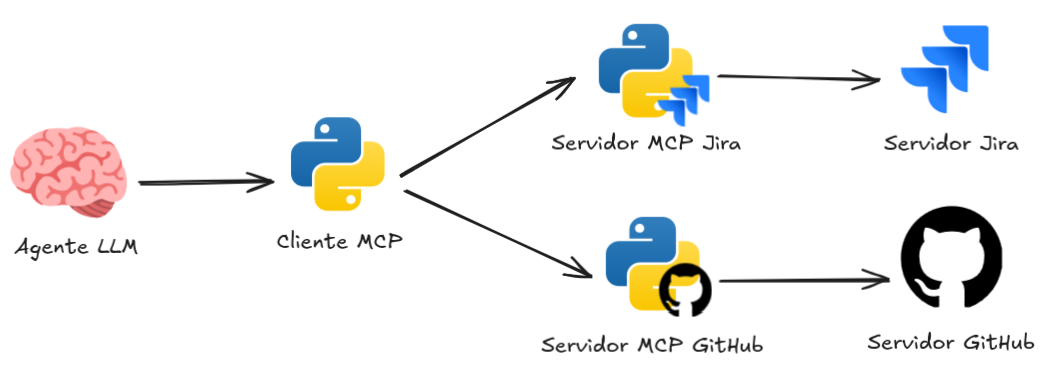
\includegraphics[width=1\linewidth]{figures/mcp.png}
  \caption{Esquema de funcionamiento del Model Context Protocol.}
  \label{fig:mcp}
\end{figure}

El protocolo ofrece dos modos de operación para la comunicación entre cliente y servidor: 
\begin{itemize}
  \item{\textbf{Comunicación SSE: }}
\end{itemize}


